\documentclass[12pt,a4paper]{report}

\usepackage[T1]{fontenc}
\usepackage[utf8]{inputenc}
\usepackage[french]{babel}
\addto\captionsfrench{%
\renewcommand{\contentsname}{Sommaire}%
\renewcommand{\listfigurename}{Liste des figures}%
\renewcommand{\listtablename}{Liste des tableaux}%
}
\usepackage{lmodern}
\usepackage{textcomp}

\usepackage[a4paper,margin=2.5cm]{geometry}
\usepackage{xcolor}
\usepackage{graphicx}
\usepackage{booktabs}
\usepackage{longtable}
\usepackage{array}
\usepackage{tabularx}
\usepackage{colortbl}
\usepackage{float}
\usepackage{ragged2e}
\usepackage{listings}
\usepackage{titlesec}
\usepackage{fancyhdr}
\usepackage{caption}
\usepackage{amssymb}
\usepackage{hyperref}

\definecolor{bleu}{RGB}{35,44,61}     % #232C3D  indigo (titres, en-têtes)
\definecolor{or}{RGB}{198,138,61}    % #C68A3D  ocre banco (accents, étoiles)
\definecolor{laterite}{RGB}{168,70,47} % #A8462F latérite (liens externes)
\definecolor{grisfond}{RGB}{247,247,247}

\graphicspath{{images/}}

\hypersetup{
colorlinks=true,
linkcolor=bleu,
urlcolor=laterite,
citecolor=bleu,
pdftitle={Manuel d'utilisation - Application Environnement du Burkina Faso},
pdfauthor={KOUMTOUBRE Tuwendé Davy Donald, KANIHE Bougapiou Anderson},
pdfsubject={Web Sémantique et Web de Données - IBAM/UJKZ},
}

\captionsetup{labelfont=bf, font=footnotesize, labelsep=endash}

\titleformat{\chapter}[hang]{\normalfont\bfseries\color{bleu}}
{\fontsize{45}{50}\selectfont\thechapter}{0.6em}{\Huge}
\titlespacing*{\chapter}{0pt}{-38pt}{28pt}

\titleformat{\section}{\normalfont\Large\bfseries\color{bleu}}{\thesection}{0.8em}{}
\titlespacing*{\section}{0pt}{18pt}{8pt}

\titleformat{\subsection}{\normalfont\large\bfseries\color{bleu}}{\thesubsection}{0.8em}{}
\titlespacing*{\subsection}{0pt}{12pt}{6pt}

\renewcommand{\chaptermark}[1]{\markboth{#1}{}}
\pagestyle{fancy}
\fancyhf{}
\fancyhead[L]{\footnotesize\itshape\nouppercase{Chapitre~\leftmark}}
\fancyfoot[C]{\thepage}
\renewcommand{\headrulewidth}{0pt}

\lstset{
basicstyle=\ttfamily\footnotesize,
frame=single,
framerule=0.3pt,
rulecolor=\color{gray!60},
backgroundcolor=\color{gray!5},
breaklines=true,
showstringspaces=false,
columns=flexible,
literate={à}{{\`a}}1 {é}{{\'e}}1 {è}{{\`e}}1 {ê}{{\^e}}1 {ô}{{\^o}}1 {û}{{\^u}}1 {ç}{{\c{c}}}1 {«}{{\guillemotleft}}1 {»}{{\guillemotright}}1,
}

\newcommand{\tete}[1]{\cellcolor{bleu}\textcolor{white}{\bfseries #1}}

\begin{document}

% ======================= PAGE DE GARDE =======================
\begin{titlepage}
\thispagestyle{empty}
\centering

\includegraphics[width=2.6cm]{ujkz.png}\par
\vspace{0.6em}
{\LARGE\bfseries UNIVERSITÉ JOSEPH KI-ZERBO}\par
\vspace{0.15em}
{\large (UJKZ)}\par
\vspace{0.8em}
{\Large\bfseries\color{or}$\star\star\star\star\star$}\par
\vspace{1.4em}
{\LARGE\bfseries INSTITUT BURKINABÈ DES ARTS ET MÉTIERS}\par
\vspace{0.15em}
{\large (IBAM)}\par
\vspace{2.2em}
{\large Cours : Web Sémantique et Web de Données}\par
\vspace{2.6em}
{\Large\bfseries\color{bleu} MANUEL D'UTILISATION}\par
\vspace{1.6em}
{\large\bfseries Application de découverte de l'environnement du Burkina Faso}\par
\vspace{0.3em}
{\large Modélisation de l'ontologie du domaine « Faune du Burkina Faso »}\par
\vspace{0.3em}
{\large Lot : Environnement}\par
\vspace{2.6em}
{\normalsize\bfseries Groupe N\textsuperscript{o} 25}\par
\vspace{0.2em}
{\normalsize KOUMTOUBRE Tuwendé Davy Donald \hspace{4.5em}(Option ISIE)}\par
{\normalsize KANIHE Bougapiou Anderson \hspace{4.5em}(Option SI)}\par
\vspace{3em}
{\large Encadré par}\par
\vspace{0.1em}
{\large\bfseries Dr. GUINKO T. Ferdinand}\par
\vspace{3em}
{\large Date de soumission : 17/08/2026}\par
\vspace{0.2em}
{\large Année universitaire 2025--2026}\par
\end{titlepage}

\pagenumbering{roman}

\tableofcontents
\listoffigures
\listoftables

\chapter*{Liste des sigles et abréviations}
\addcontentsline{toc}{chapter}{Liste des sigles et abréviations}
\renewcommand{\thetable}{\arabic{table}}
\begin{table}[H]
\centering
\caption{Liste des sigles et abréviations}
\begin{tabular}{@{}p{3.4cm}p{11.6cm}@{}}
\hline
\tete{Sigle} & \tete{Signification} \\
\hline
\rowcolor{grisfond} API & Application Programming Interface (interface de programmation) \\
\rowcolor{grisfond} CR & En danger critique d'extinction (UICN, statut \textit{Critically Endangered}) \\
\rowcolor{grisfond} EN & En danger (UICN, statut \textit{Endangered}) \\
\rowcolor{grisfond} Flask & Micro-framework web Python utilisé pour l'application \\
\rowcolor{grisfond} GeoSPARQL & Extension géospatiale du langage de requête SPARQL \\
\rowcolor{grisfond} IRI & \textit{Internationalized Resource Identifier} (identifiant de ressource) \\
\rowcolor{grisfond} LC & Préoccupation mineure (UICN, statut \textit{Least Concern}) \\
\rowcolor{grisfond} OWL & \textit{Web Ontology Language} (langage de représentation d'ontologies) \\
\rowcolor{grisfond} RDF & \textit{Resource Description Framework} \\
\rowcolor{grisfond} SPARQL & Langage de requête pour interroger des données RDF \\
\rowcolor{grisfond} SWRL & \textit{Semantic Web Rule Language} (langage de règles) \\
\rowcolor{grisfond} TDB2 & Base de données native de stockage de graphes RDF (Jena) \\
\rowcolor{grisfond} UICN & Union internationale pour la conservation de la nature \\
\rowcolor{grisfond} OWL/XML & Syntaxe XML du langage OWL (fichiers ``\texttt{.owx}'') \\
\rowcolor{grisfond} RDF/XML & Syntaxe XML de RDF (fichiers ``\texttt{.rdf}'') \\
\hline
\end{tabular}
\end{table}
\renewcommand{\thetable}{\thechapter.\arabic{table}}

\pagenumbering{arabic}

% ======================= CHAPITRE 1 =======================
\chapter{Introduction}

\section{Présentation de l'application}

L'application \textbf{« Environnement du Burkina Faso »} est une plateforme sémantique web permettant
d'explorer la faune, la flore, le réseau hydrographique et les localités du Burkina Faso. Toutes les
données affichées proviennent de l'ontologie OWL~2 \textit{« burkina-environnement »} (55 classes,
1\,598 individus), interrogeable en SPARQL et GeoSPARQL via le triplestore \textbf{Apache Jena Fuseki}.

\section{Architecture technique}

\begin{itemize}
\item \textbf{Base de connaissances} : l'ontologie est chargée dans un jeu de données Fuseki nommé
\texttt{environnement}, sous les formats \url{ontologie_environnement.owx} ou
\url{ontologie_environnement.rdf}.
\item \textbf{Back-end} : une application \textbf{Flask} (Python) exécute des requêtes SPARQL sur le
triplestore et expose des \emph{APIs JSON} à l'interface.
\item \textbf{Front-end} : une interface web HTML/CSS/JavaScript (sans framework), avec la
bibliothèque cartographique \textbf{Leaflet} / OpenStreetMap pour la carte spatiale.
\end{itemize}

\begin{figure}[htbp]
\centering
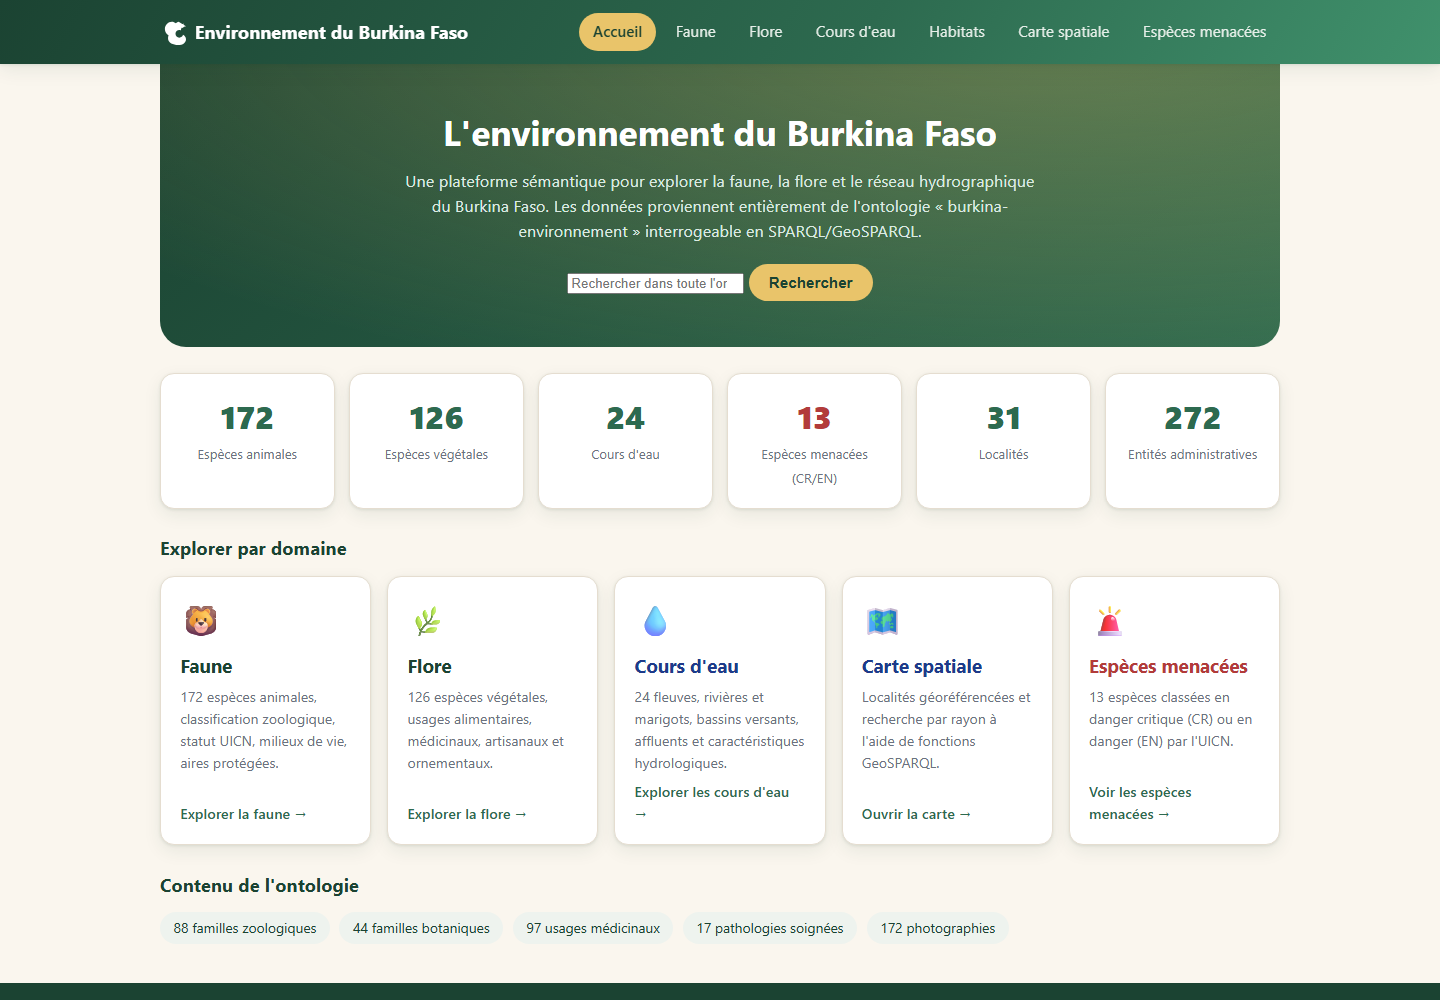
\includegraphics[width=0.82\textwidth]{01_accueil.png}
\caption[Page d'accueil de l'application]{Vue d'ensemble de la page d'accueil : bandeau de navigation, moteur de recherche globale et
compteurs statistiques de l'application.}
\end{figure}

\section{Contenu du dossier livré}

Le projet à déployer contient les fichiers et dossiers suivants :

\begin{table}[H]
\centering
\caption{Contenu du dossier livré}
\begin{tabular}{@{}p{5.8cm}p{9.2cm}@{}}
\hline
\tete{Élément} & \tete{Rôle} \\
\hline
\rowcolor{grisfond} \texttt{app.py} & Point d'entrée de l'application Flask \\
\rowcolor{grisfond} \texttt{requirements.txt} & Liste des dépendances Python à installer \\
\rowcolor{grisfond} \url{ontologie_environnement.owx} & Ontologie au format OWL/XML (à charger dans Fuseki) \\
\rowcolor{grisfond} \url{ontologie_environnement.rdf} & Ontologie au format RDF/XML (équivalente) \\
\rowcolor{grisfond} \texttt{backend/} & Requêtes SPARQL et logique métier (faune, flore, cours d'eau, habitats, statistiques) \\
\rowcolor{grisfond} \texttt{web/} & Blueprints Flask (routes des pages et des APIs) \\
\rowcolor{grisfond} \texttt{templates/} & Gabarits HTML (Jinja2) \\
\rowcolor{grisfond} \texttt{static/} & Feuille de style CSS et scripts JavaScript \\
\hline
\end{tabular}
\end{table}

\section{Organisation du manuel}

Ce manuel guide le lecteur pas à pas : les prérequis (chapitre~2), l'installation du serveur de données
Fuseki (chapitre~3), l'installation et le lancement de l'application web (chapitre~4), puis un guide
d'utilisation détaillé avec captures d'écran (chapitre~5). Le chapitre~6 recense les problèmes
fréquents et leurs solutions.

% ======================= CHAPITRE 2 =======================
\chapter{Prérequis}

\section{Matériel et logiciels}

L'application est multiplateforme. Elle s'installe de la même manière sous Windows, Linux et macOS.

\begin{table}[H]
\centering
\caption{Prérequis matériels et logiciels}
\begin{tabular}{@{}p{4.0cm}p{5.8cm}p{4.8cm}@{}}
\hline
\tete{Logiciel} & \tete{Version minimale} & \tete{Utilité} \\
\hline
\rowcolor{grisfond} \texttt{Java} (OpenJDK / Oracle) & 17 ou plus & Exécuter Apache Jena Fuseki \\
\rowcolor{grisfond} Apache Jena Fuseki & 5.x (serveur) & Triplestore SPARQL/GeoSPARQL \\
\rowcolor{grisfond} Python & 3.10 ou plus & Exécuter l'application Flask \\
\rowcolor{grisfond} \texttt{pip} & fourni avec Python & Installer les dépendances \\
\rowcolor{grisfond} Navigateur web & récent (Chrome, Edge, Firefox) & Consulter l'application \\
\rowcolor{grisfond} Connexion Internet & au moins au premier chargement & Tuiles de la carte OpenStreetMap \\
\hline
\end{tabular}
\end{table}

\section{Vérifier les versions installées}

Ouvrir un terminal (PowerShell sous Windows, Terminal sous Linux/macOS) et exécuter :

\begin{lstlisting}
python --version
java -version
\end{lstlisting}

Si Python n'est pas reconnu, le réinstaller en activant l'option
\textbf{« Add Python to PATH »}. Si \texttt{java} n'est pas reconnu, se reporter au chapitre~3.

\section{Récupérer le dossier du projet}

Copier l'intégralité du dossier \texttt{app\_web\_semanique} sur la machine cible
(par exemple sur le Bureau). Vérifier la présence de \texttt{app.py},
\texttt{requirements.txt} et des fichiers \url{ontologie_environnement.owx} et
\url{ontologie_environnement.rdf}.

% ======================= CHAPITRE 3 =======================
\chapter{Installation du serveur de données (Jena Fuseki)}

L'application ne fonctionne que si le triplestore Fuseki, contenant l'ontologie, est démarré
\textbf{avant} l'application web.

\section{Installer Java}

\textbf{Windows} -- Télécharger un JDK 17+ (par exemple \href{https://adoptium.net}{\texttt{adoptium.net}}),
l'installer, puis vérifier avec \texttt{java -version} dans un nouveau terminal.

\textbf{Linux} -- Utiliser le gestionnaire de paquets :

\begin{lstlisting}
# Debian / Ubuntu
sudo apt install openjdk-17-jre

# Fedora
sudo dnf install java-17-openjdk
\end{lstlisting}

\textbf{macOS} -- Avec Homebrew :

\begin{lstlisting}
brew install openjdk@17
\end{lstlisting}

\section{Télécharger et démarrer Fuseki}

Télécharger \texttt{apache-jena-fuseki} depuis \href{https://jena.apache.org/download/}{\texttt{jena.apache.org/download/}}.
Décompresser l'archive, puis, dans un terminal placé dans le dossier décompressé :

\begin{lstlisting}
# Windows
fuseki-server.bat

# Linux / macOS
./fuseki-server
\end{lstlisting}

\noindent L'interface de gestion Fuseki est alors disponible à l'adresse
\url{http://localhost:3030}. Laisser ce terminal ouvert pendant toute la durée
d'utilisation de l'application.

\section{Créer le jeu de données « environnement »}

Dans l'interface Fuseki (\url{http://localhost:3030}) :

\begin{enumerate}
\item Cliquer sur \textbf{« Manage datasets »} puis sur \textbf{« add new dataset »}.
\item Saisir \textbf{environnement} dans le champ \emph{Dataset name} (nom exact, sans accent).
\item Choisir \textbf{\emph{Persistent (TDB2)}} comme type de stockage.
\item Valider avec \textbf{Create dataset}.
\end{enumerate}

\noindent Le nom du jeu de données est capital : l'application interroge précisément
\url{http://localhost:3030/environnement/query}.

\section{Charger l'ontologie}

Toujours dans l'interface Fuseki :

\begin{enumerate}
\item Ouvrir le jeu de données \textbf{environnement}.
\item Cliquer sur \textbf{« upload data »}.
\item Sélectionner le fichier \url{ontologie_environnement.owx} ou le fichier
\url{ontologie_environnement.rdf}.
\item Cliquer sur \textbf{« upload now »} et attendre la fin du chargement (quelques secondes).
\end{enumerate}

\section{Vérifier le chargement}

Dans l'onglet \textbf{Query} du jeu de données, exécuter la requête de contrôle :

\begin{lstlisting}
PREFIX en: <http://www.ibam-ujkz.bf/ontologies/burkina-environnement#>
SELECT (COUNT(?s) AS ?individus) WHERE { ?s a en:EspeceAnimale }
\end{lstlisting}

\noindent La réponse doit être proche de \texttt{172} individus (les espèces animales de l'ontologie).

% ======================= CHAPITRE 4 =======================
\chapter{Installation et lancement de l'application web}

\section{Installer les dépendances Python}

Ouvrir un terminal dans le dossier du projet (celui qui contient \texttt{app.py}) et créer un
environnement virtuel :

\textbf{Windows}

\begin{lstlisting}
cd app_web_semanique
python -m venv .venv
.venv\Scripts\activate
pip install -r requirements.txt
\end{lstlisting}

\textbf{Linux / macOS}

\begin{lstlisting}
cd app_web_semanique
python3 -m venv .venv
source .venv/bin/activate
pip install -r requirements.txt
\end{lstlisting}

\noindent Le fichier \texttt{requirements.txt} installe automatiquement :
\texttt{Flask}, \texttt{requests} et \texttt{rdflib}.

\section{Lancer l'application}

Toujours dans le terminal (environnement virtuel activé) :

\begin{lstlisting}
python app.py
\end{lstlisting}

\noindent Un message confirme le démarrage du serveur. Ouvrir ensuite le navigateur à l'adresse
\url{http://127.0.0.1:5000} : la page d'accueil de l'application doit s'afficher.

\section{Ordre de démarrage recommandé}

\begin{enumerate}
\item Démarrer Fuseki (chapitre~3) et vérifier \url{http://localhost:3030}.
\item Démarrer l'application avec \texttt{python app.py}.
\item Ouvrir \url{http://127.0.0.1:5000}.
\end{enumerate}

\section{Arrêter l'application}

Fermer l'application avec \texttt{Ctrl+C} dans son terminal. Pour arrêter Fuseki, fermer son
terminal ou utiliser \texttt{Ctrl+C}. Le jeu de données \texttt{environnement} est conservé
(stockage persistant TDB2) : il n'est pas nécessaire de recharger l'ontologie au prochain démarrage.

% ======================= CHAPITRE 5 =======================
\chapter{Guide d'utilisation}

\section{Page d'accueil}

La page d'accueil (\texttt{/}) présente six compteurs récapitulatifs alimentés par l'ontologie :
\textbf{172 espèces animales}, \textbf{126 espèces végétales}, \textbf{24 cours d'eau},
\textbf{13 espèces menacées} (statuts UICN CR/EN), \textbf{31 localités} et
\textbf{272 entités administratives}. Elle donne aussi accès aux domaines de l'application
(Faune, Flore, Cours d'eau, Carte spatiale, Espèces menacées) et contient le moteur de recherche
globale (voir §~5.2).

\begin{figure}[htbp]
\centering
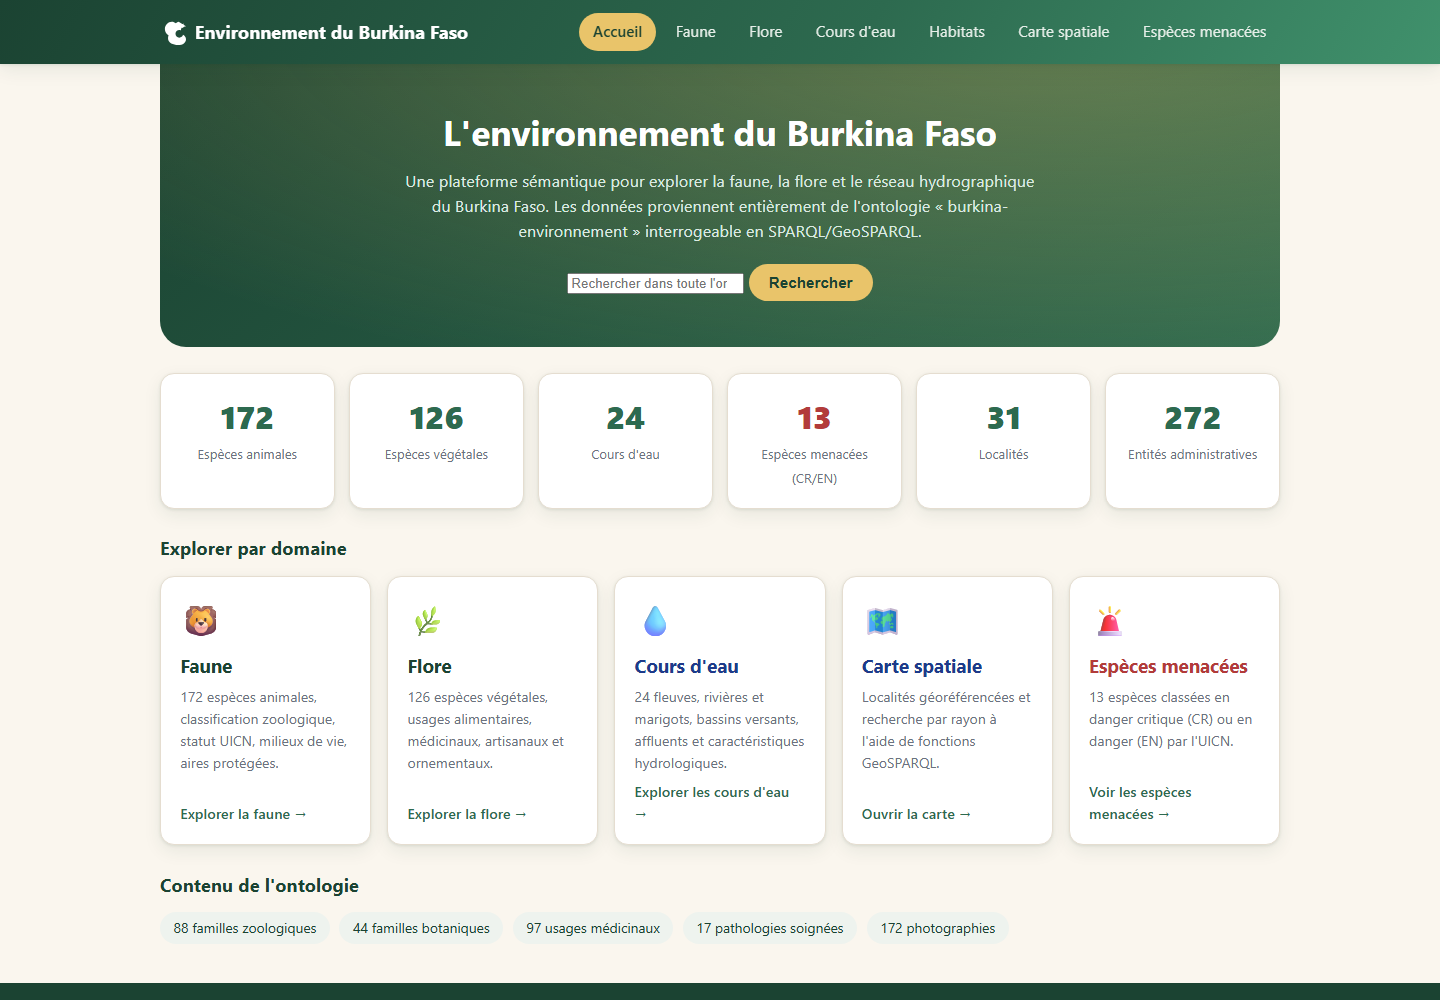
\includegraphics[width=\textwidth]{01_accueil.png}
\caption[Page d'accueil et ses compteurs statistiques]{Page d'accueil et ses six compteurs alimentés par l'ontologie : 172 espèces animales,
126 espèces végétales, 24 cours d'eau, 13 espèces menacées, 31 localités et 272 entités
administratives.}
\end{figure}

\section{Recherche globale}

Depuis la barre \textbf{Rechercher dans toute l'ontologie}, saisir au moins deux caractères : un
panneau de résultats apparaît aussitôt, mêlant espèces animales, espèces végétales, cours d'eau et
localités (habitats). Cliquer sur un résultat pour ouvrir sa fiche. La recherche est insensible aux
accents et à la casse (par exemple \texttt{guépard}, \texttt{guepard} ou \texttt{GUEPARD} donnent le
même résultat).

\begin{figure}[htbp]
\centering
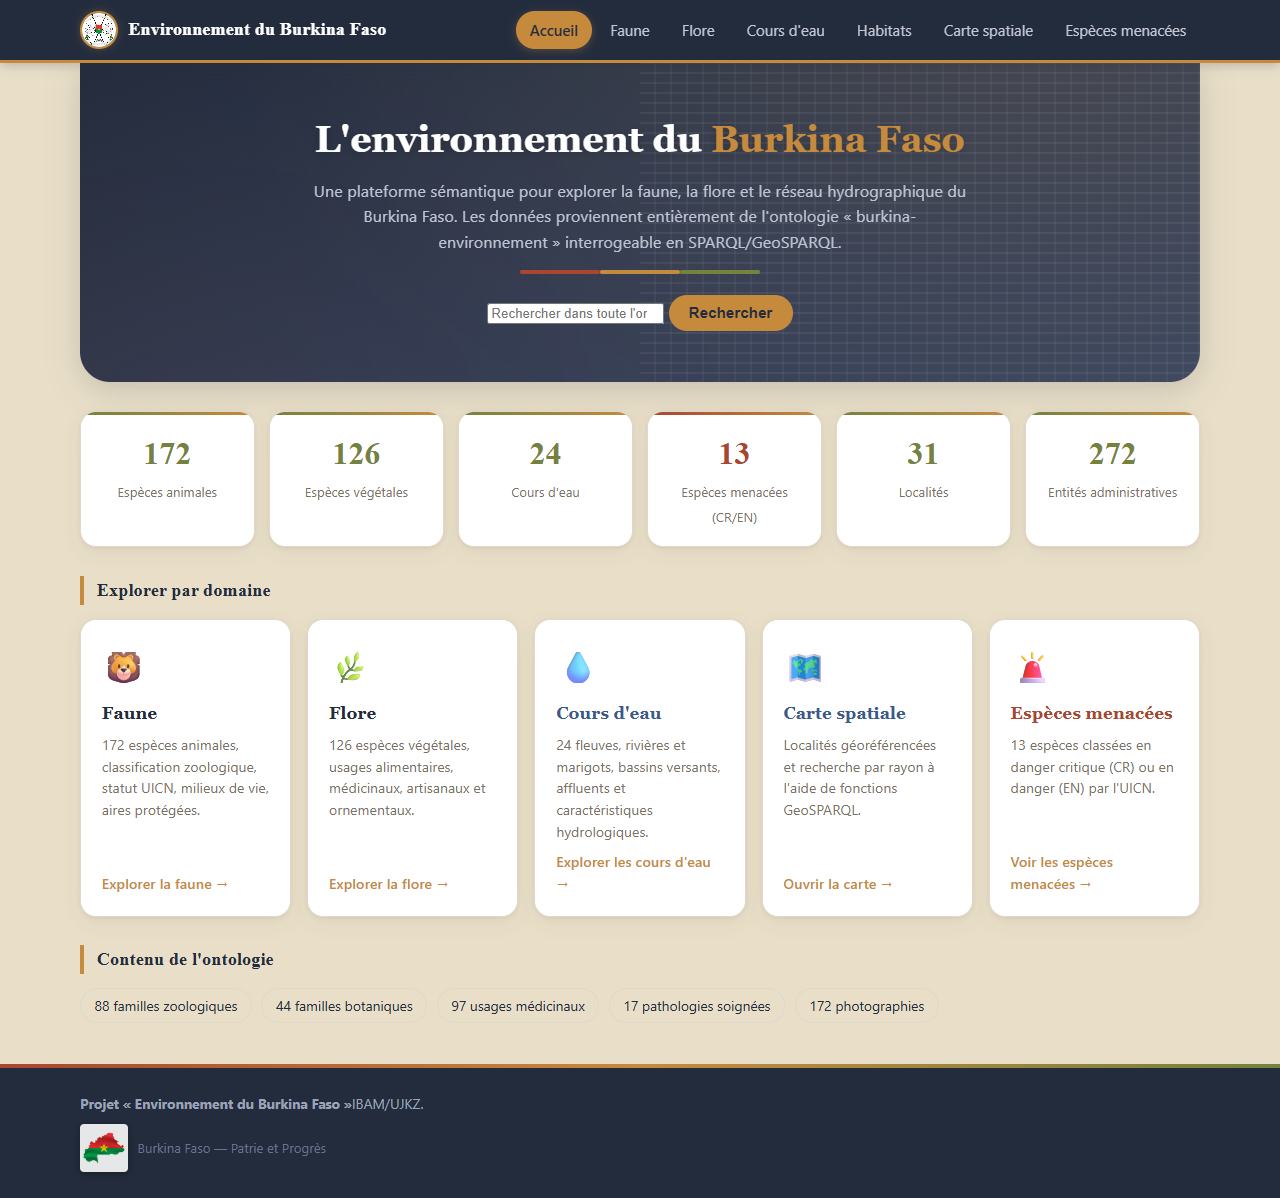
\includegraphics[width=\textwidth]{02_recherche.png}
\caption[Résultats de la recherche globale (\texttt{wayen})]{Résultats de la recherche globale pour le terme \texttt{wayen} : le panneau de résultats
mêle les types de ressources (habitat) et fournit un lien direct vers la fiche correspondante.}
\end{figure}

\section{Domaines « Faune » et « Flore »}

Les pages \texttt{/faune} et \texttt{/flore} fonctionnent de façon identique :

\begin{enumerate}
\item \textbf{Recherche} : champ texte cherchant dans les noms communs et scientifiques.
\item \textbf{Filtres} : groupe zoologique (respectivement famille botanique), famille, milieu de
vie, statut UICN et localité d'observation.
\item \textbf{Liste} : cartes d'aperçu (photo, nom, statut), avec pagination (10 éléments par page)
et compteur « affichées sur total ».
\end{enumerate}

\begin{figure}[htbp]
\centering
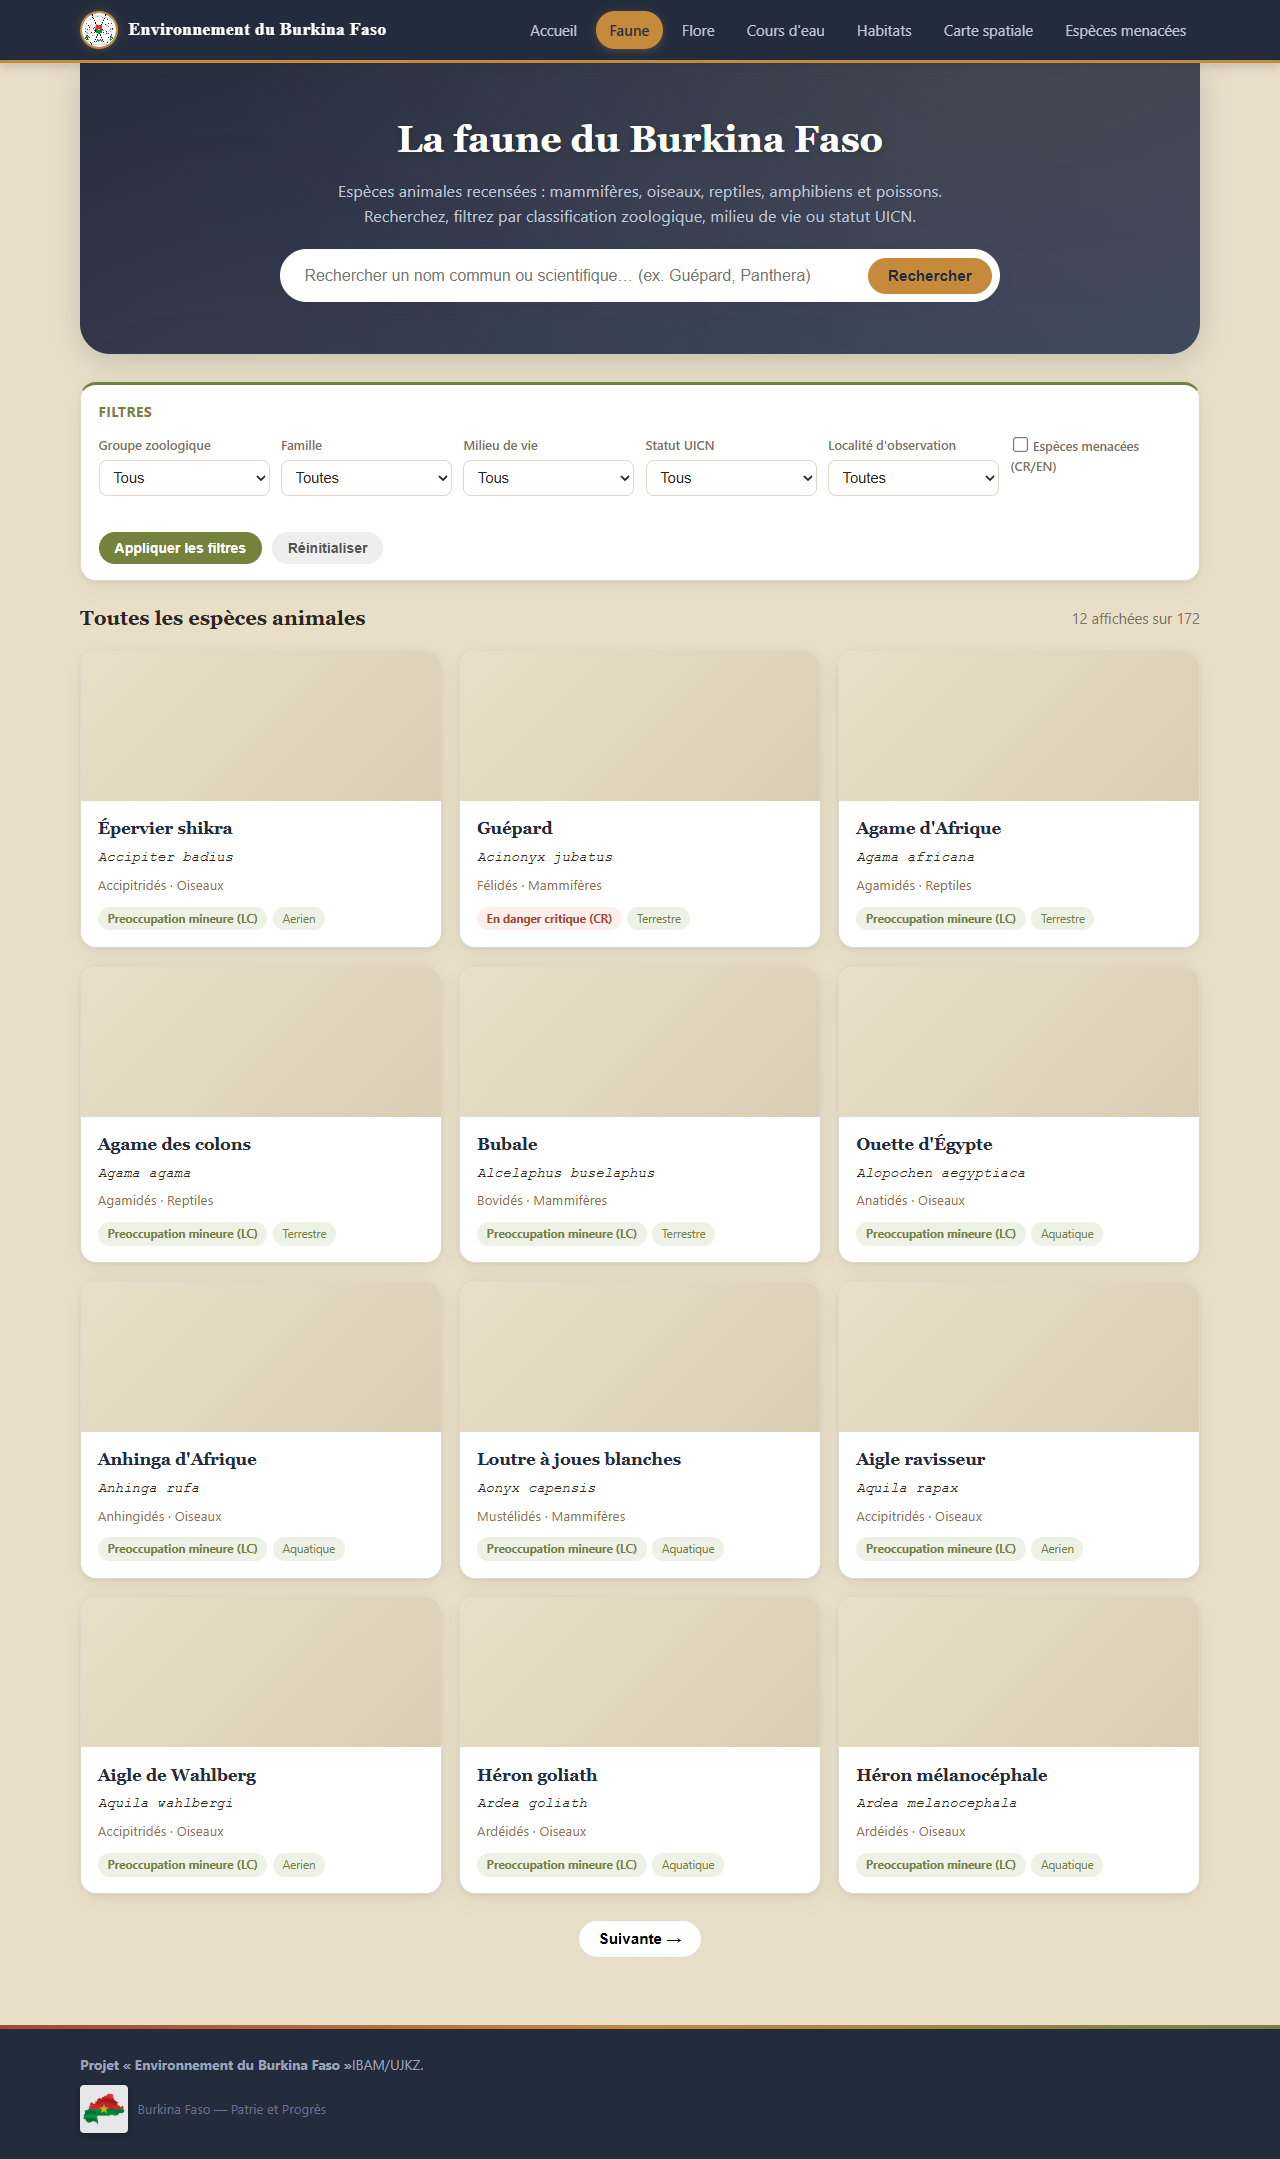
\includegraphics[width=\textwidth]{03_faune.png}
\caption[Page « Faune » : recherche, filtres et liste d'espèces]{Page « Faune » : champ de recherche, panneau de filtres (groupe zoologique, famille, milieu
de vie, statut UICN, localité) et liste paginée de cartes d'aperçu des espèces.}
\end{figure}

\begin{figure}[htbp]
\centering
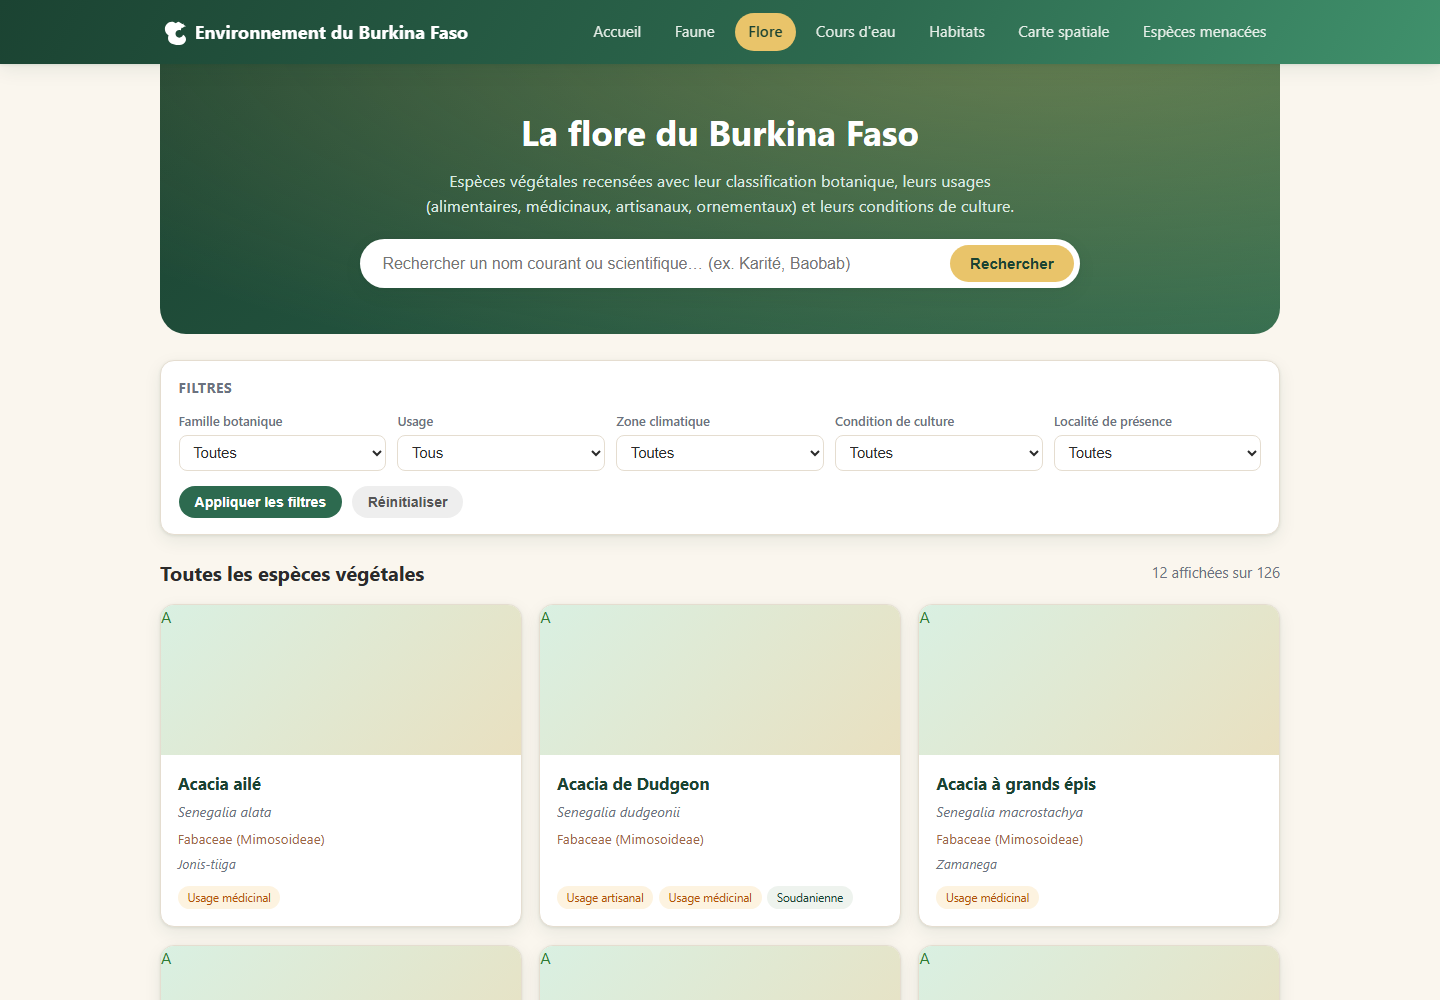
\includegraphics[width=\textwidth]{05_flore.png}
\caption[Page « Flore » avec ses filtres]{Page « Flore » : mêmes mécanismes que la faune (recherche, filtres par famille botanique,
statut UICN et localité), avec les cartes d'aperçu des espèces végétales.}
\end{figure}

\section{Les fiches}

En cliquant sur un élément, sa fiche détaillée s'affiche.

\textbf{Fiche espèce animale} (\texttt{/faune/<nom>}) : photo, nom commun et nom scientifique, statut
UICN, description, classification zoologique complète, caractéristiques (régime alimentaire, poids,
durée de vie), milieux de vie, zones d'observation (liens vers les habitats) et source.

\begin{figure}[htbp]
\centering
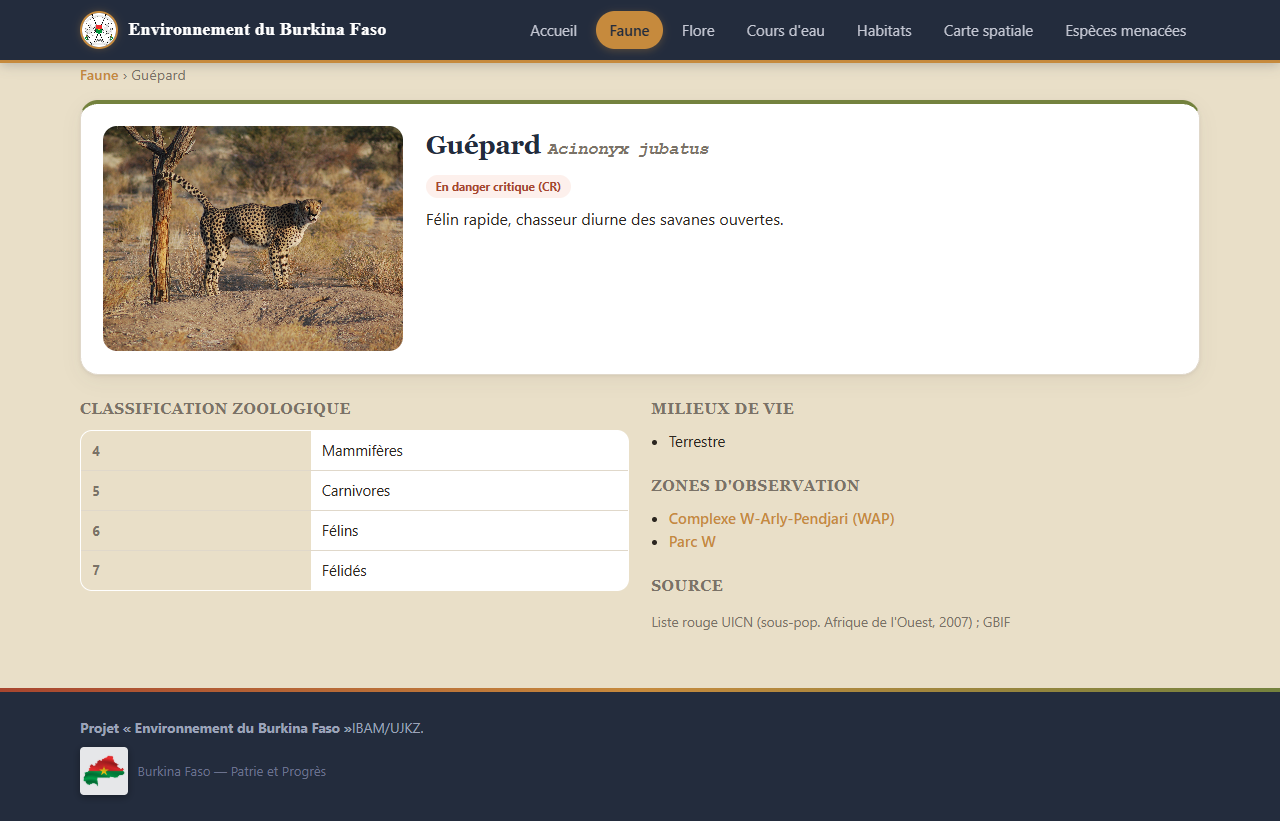
\includegraphics[width=\textwidth]{04_fiche_faune.png}
\caption[Fiche de l'espèce \textit{Acinonyx jubatus} (Guépard)]{Fiche détaillée d'une espèce animale (exemple : le Guépard, \textit{Acinonyx jubatus}) :
photo, statut UICN, classification zoologique, caractéristiques, milieux de vie et zones
d'observation.}
\end{figure}

\textbf{Fiche espèce végétale} (\texttt{/flore/<nom>}) : classification botanique, caractéristiques,
localités de présence, précautions éventuelles, usages (alimentaires, médicinaux, artisanaux,
ornementaux) et source.

\begin{figure}[htbp]
\centering
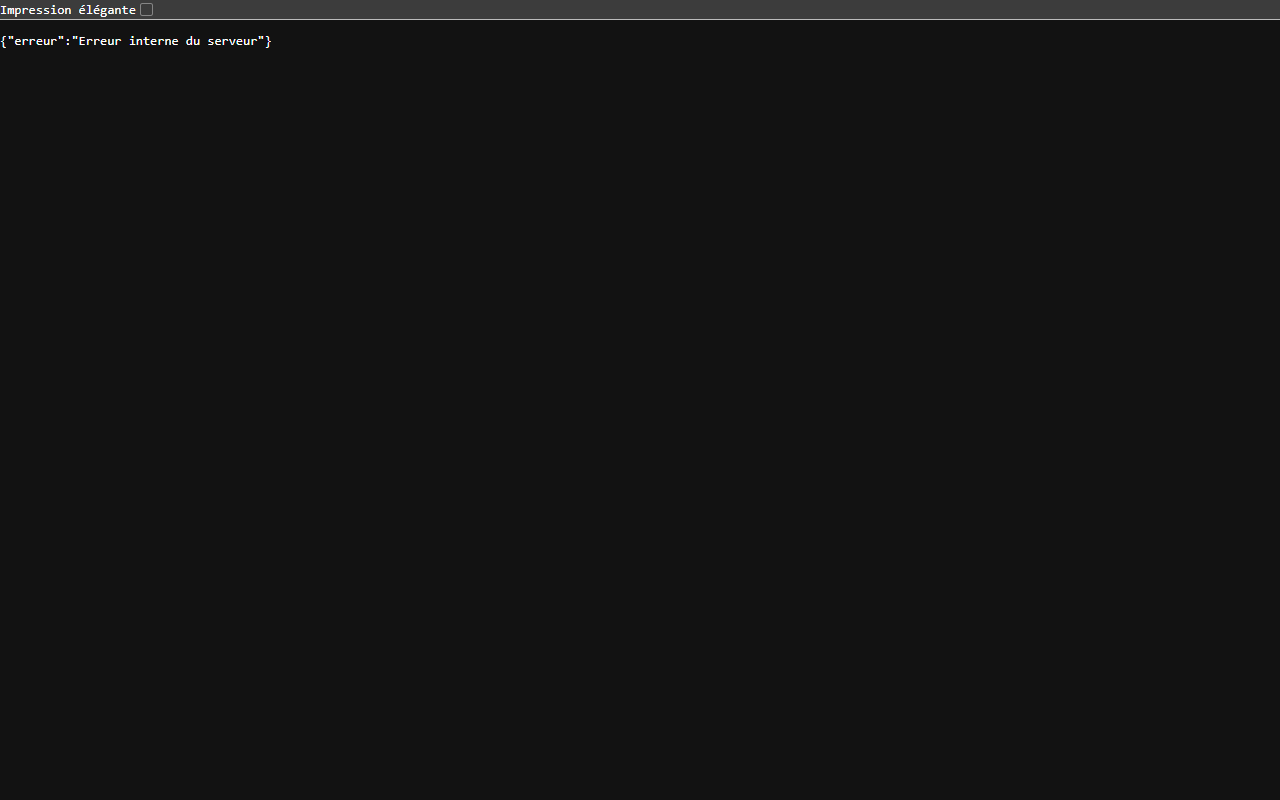
\includegraphics[width=\textwidth]{06_fiche_flore.png}
\caption[Fiche de l'espèce \textit{Vitellaria paradoxa} (Karité)]{Fiche détaillée d'une espèce végétale (exemple : le Karité, \textit{Vitellaria paradoxa}) :
classification botanique, caractéristiques, usages alimentaires ou médicinaux et localités de
présence.}
\end{figure}

\section{Cours d'eau}

La page \texttt{/cours-deau} recense les 24 cours d'eau (3 fleuves, 20 rivières et 1 marigot).
On peut rechercher et filtrer par type (Fleuve, Rivière, Marigot). La fiche (\texttt{/cours-deau/<nom>})
détaille le type, le bassin versant, la longueur, les affluents, les caractéristiques hydrologiques,
le parcours, les entités traversées et les peuples associés.

\begin{figure}[htbp]
\centering
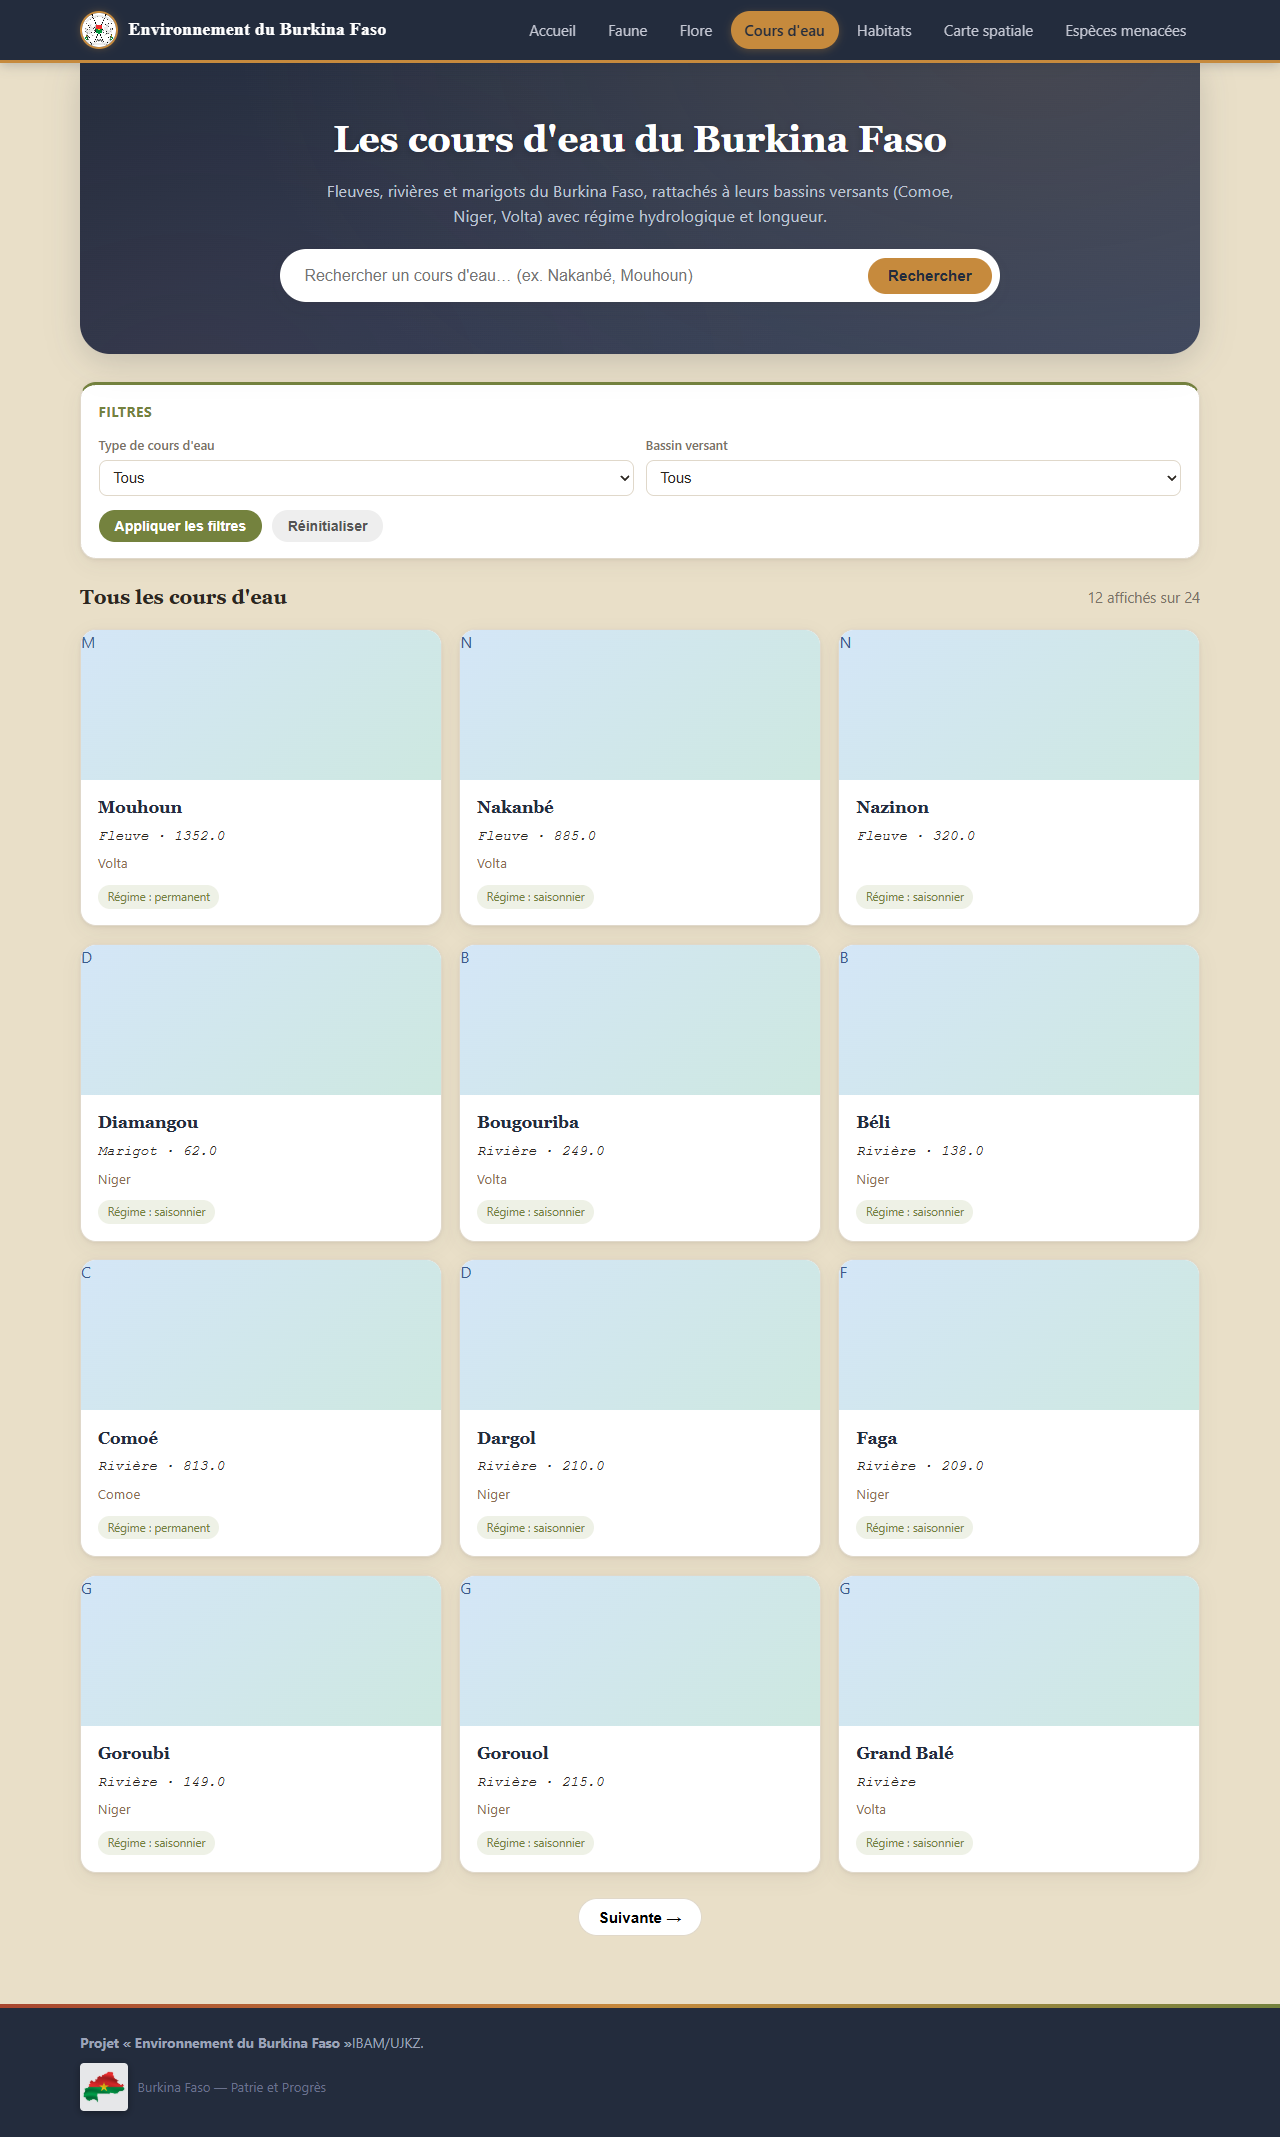
\includegraphics[width=\textwidth]{07_cours_deau.png}
\caption[Page « Cours d'eau » avec filtre par type]{Page « Cours d'eau » : liste des 24 cours d'eau avec le filtre par type (Fleuve, Rivière,
Marigot) et la recherche par nom.}
\end{figure}

\begin{figure}[htbp]
\centering
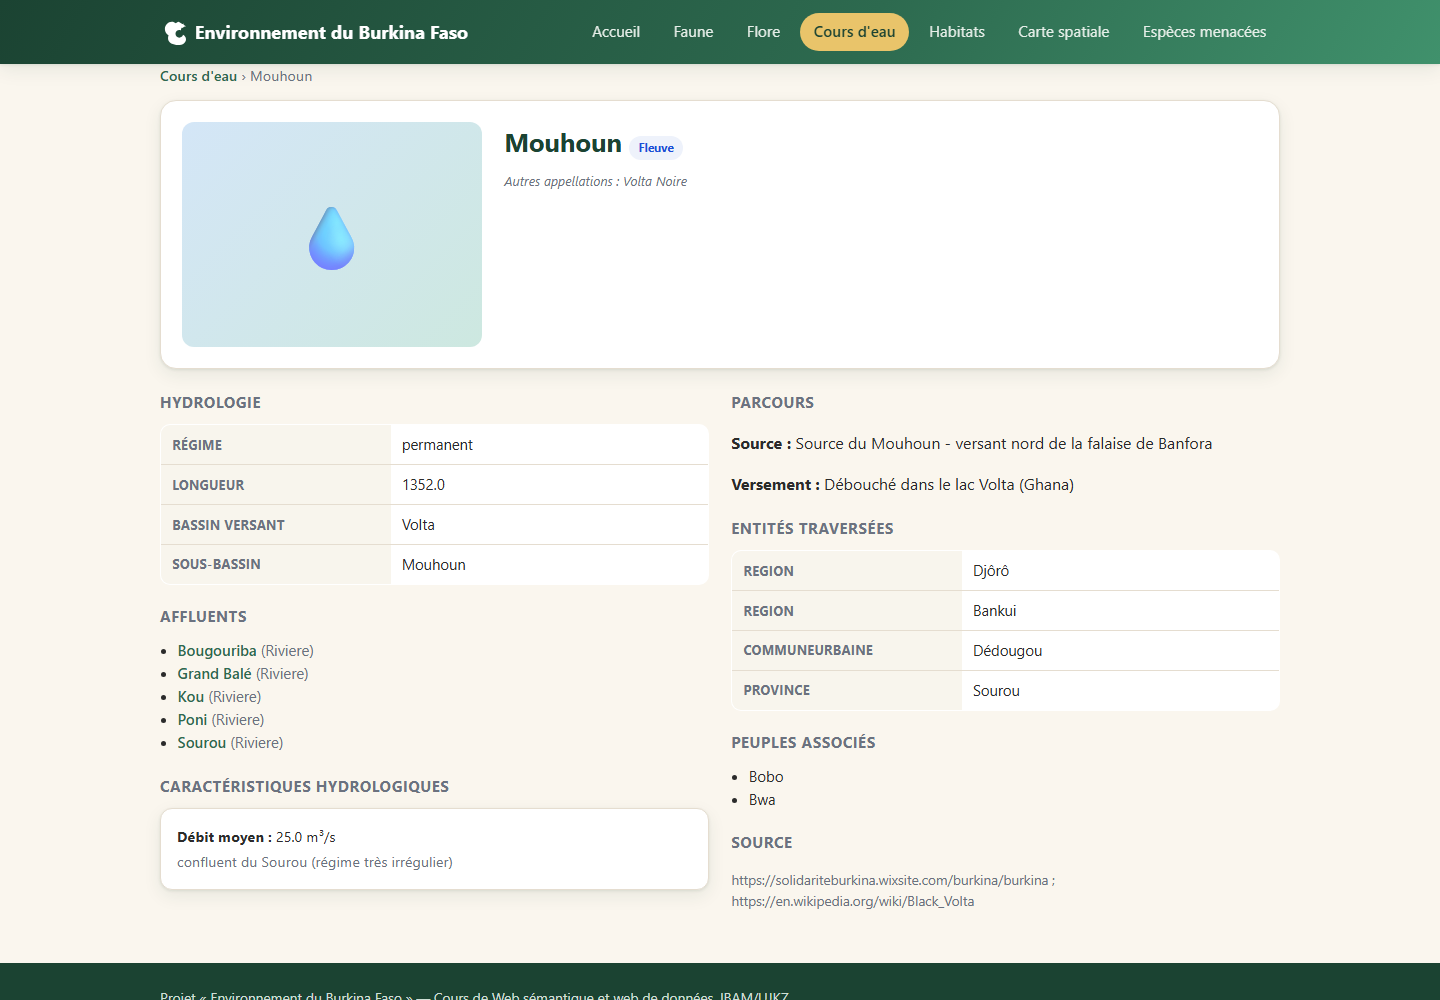
\includegraphics[width=\textwidth]{08_fiche_cours_deau.png}
\caption[Fiche du fleuve Mouhoun]{Fiche d'un cours d'eau (exemple : le fleuve Mouhoun) : type, bassin versant, longueur,
affluents, parcours et entités traversées.}
\end{figure}

\section{Habitats (localités)}

La page \texttt{/habitats} liste les 31 localités du Burkina Faso (parcs, réserves, zones humides,
localités urbaines). Sa fiche (\texttt{/habitats/<nom>}) présente la faune présente, la flore
présente et les cours d'eau associés, chaque liste étant cliquable.

\begin{figure}[htbp]
\centering
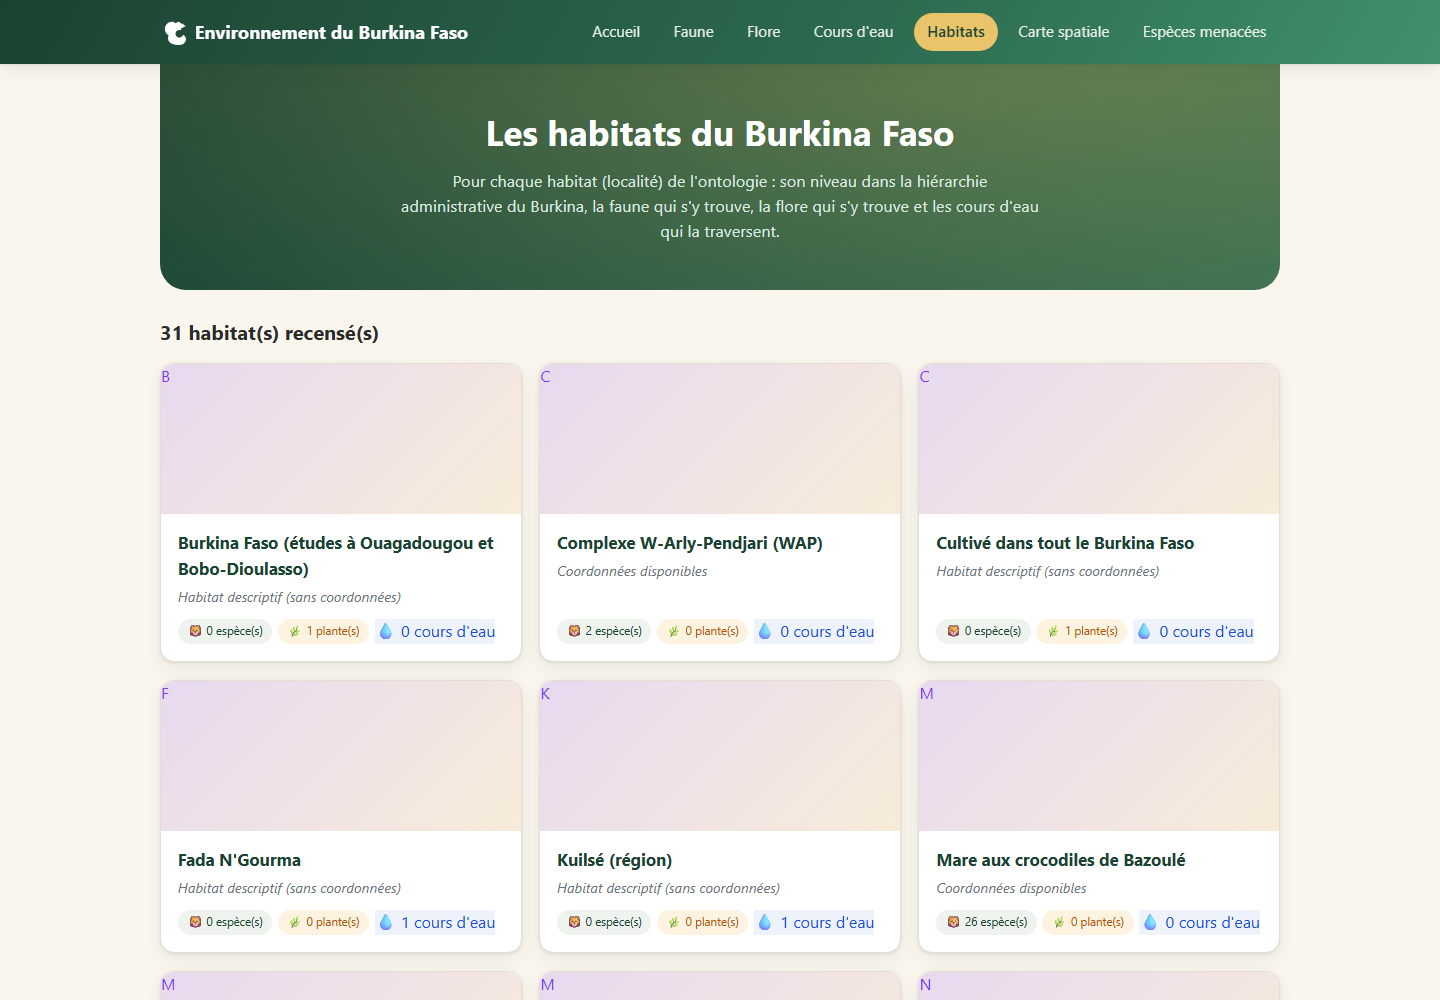
\includegraphics[width=\textwidth]{09_habitats.png}
\caption[Page « Habitats » : liste des localités]{Page « Habitats » : liste paginée des 31 localités du Burkina Faso (parcs, réserves, zones
humides, localités urbaines), avec recherche par nom.}
\end{figure}

\begin{figure}[htbp]
\centering
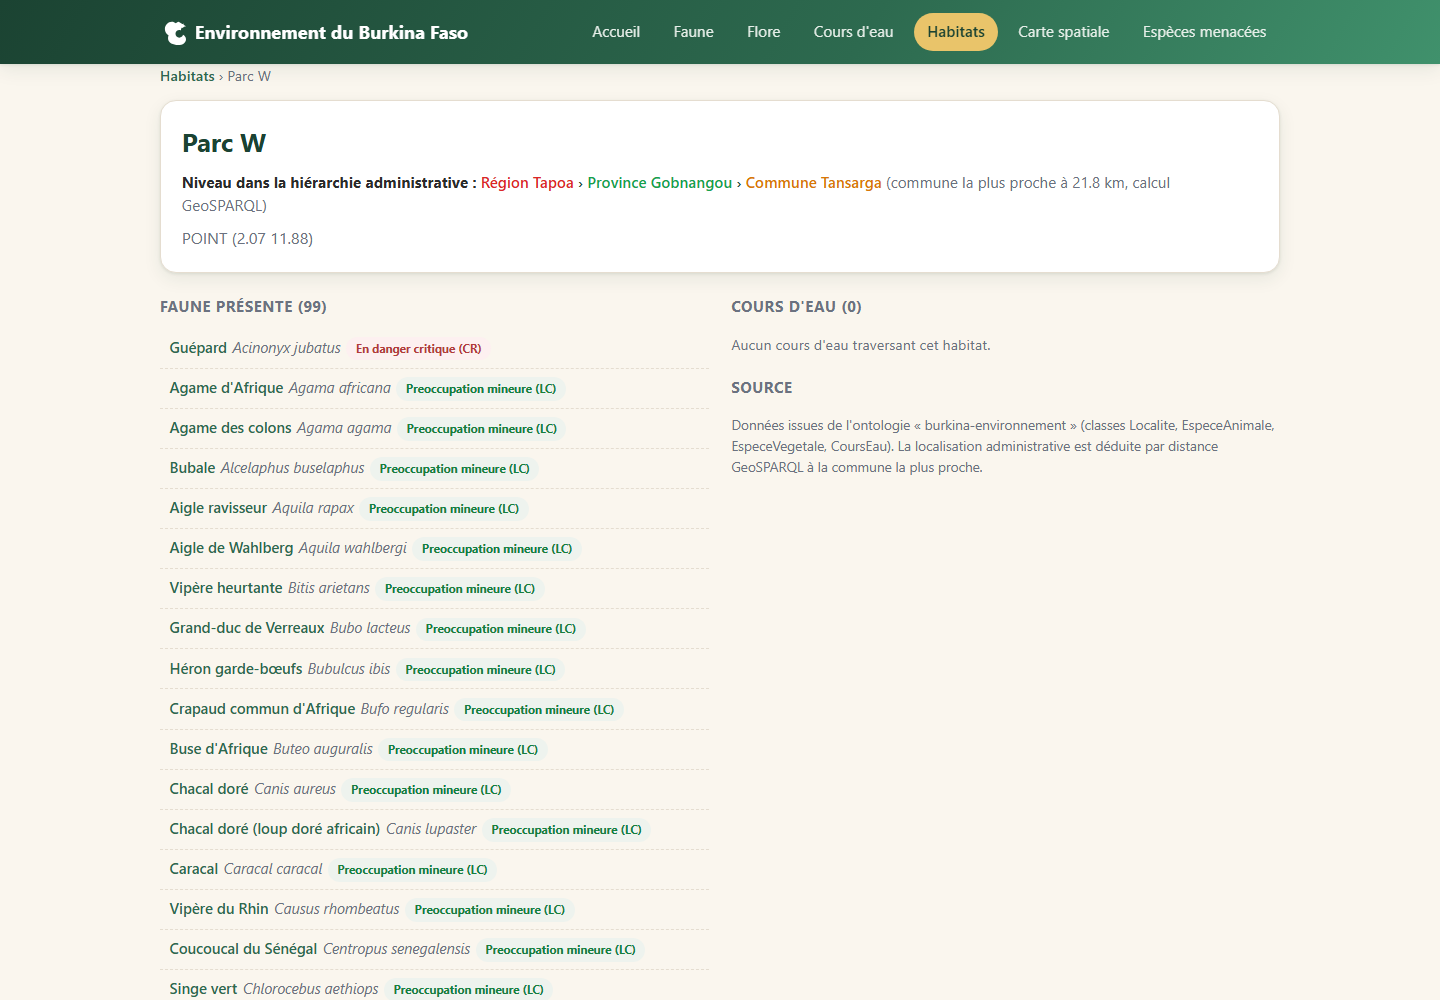
\includegraphics[width=\textwidth]{10_fiche_habitat.png}
\caption[Fiche du Parc W]{Fiche d'une localité (exemple : le Parc W) : faune présente, flore présente et cours d'eau
associés, chaque liste étant cliquable pour ouvrir les fiches correspondantes.}
\end{figure}

\section{Carte spatiale}

La page \texttt{/carte} utilise Leaflet et OpenStreetMap. Les 31 localités sont géoréférencées sur
la carte ; une couche optionnelle affiche les 272 entités administratives (régions, provinces,
communes). La fonction \textbf{Recherche par rayon} (GeoSPARQL) permet de cliquer sur la carte puis
de saisir un rayon (en kilomètres) pour lister les localités alentour.

\begin{figure}[htbp]
\centering
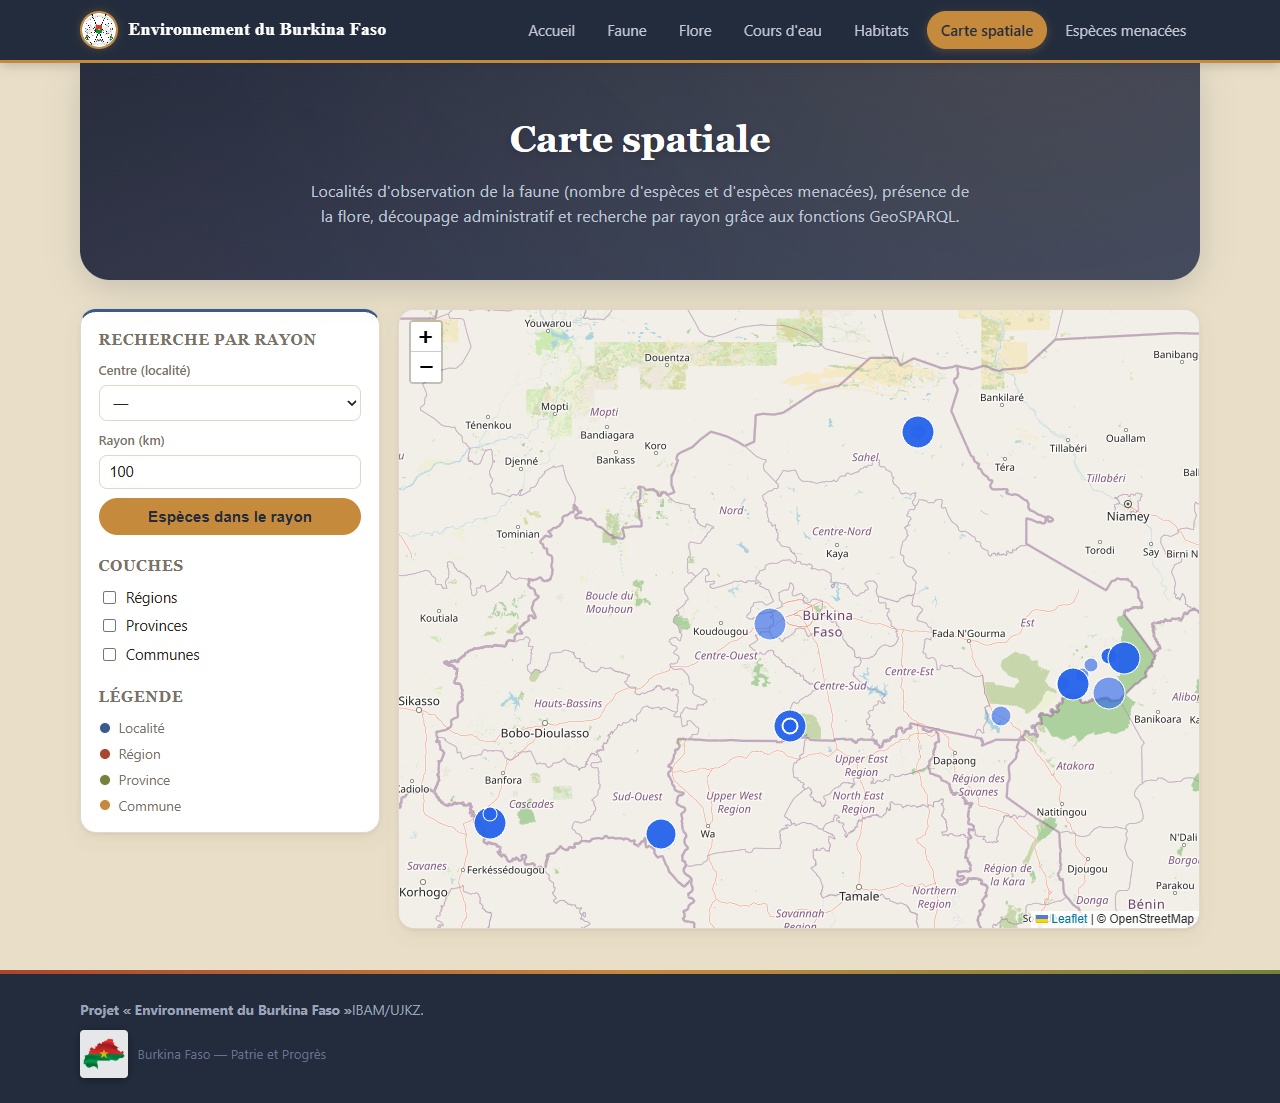
\includegraphics[width=\textwidth]{11_carte.png}
\caption[Carte spatiale : localités et recherche par rayon]{Carte spatiale Leaflet/OpenStreetMap : les 31 localités géoréférencées, la couche des
272 entités administratives et l'outil de recherche par rayon (GeoSPARQL).}
\end{figure}

\section{Espèces menacées}

La page \texttt{/menacees} liste les 13 espèces animales en danger critique (CR) ou en danger (EN)
selon la classification UICN, avec leur statut affiché en badge coloré.

\begin{figure}[htbp]
\centering
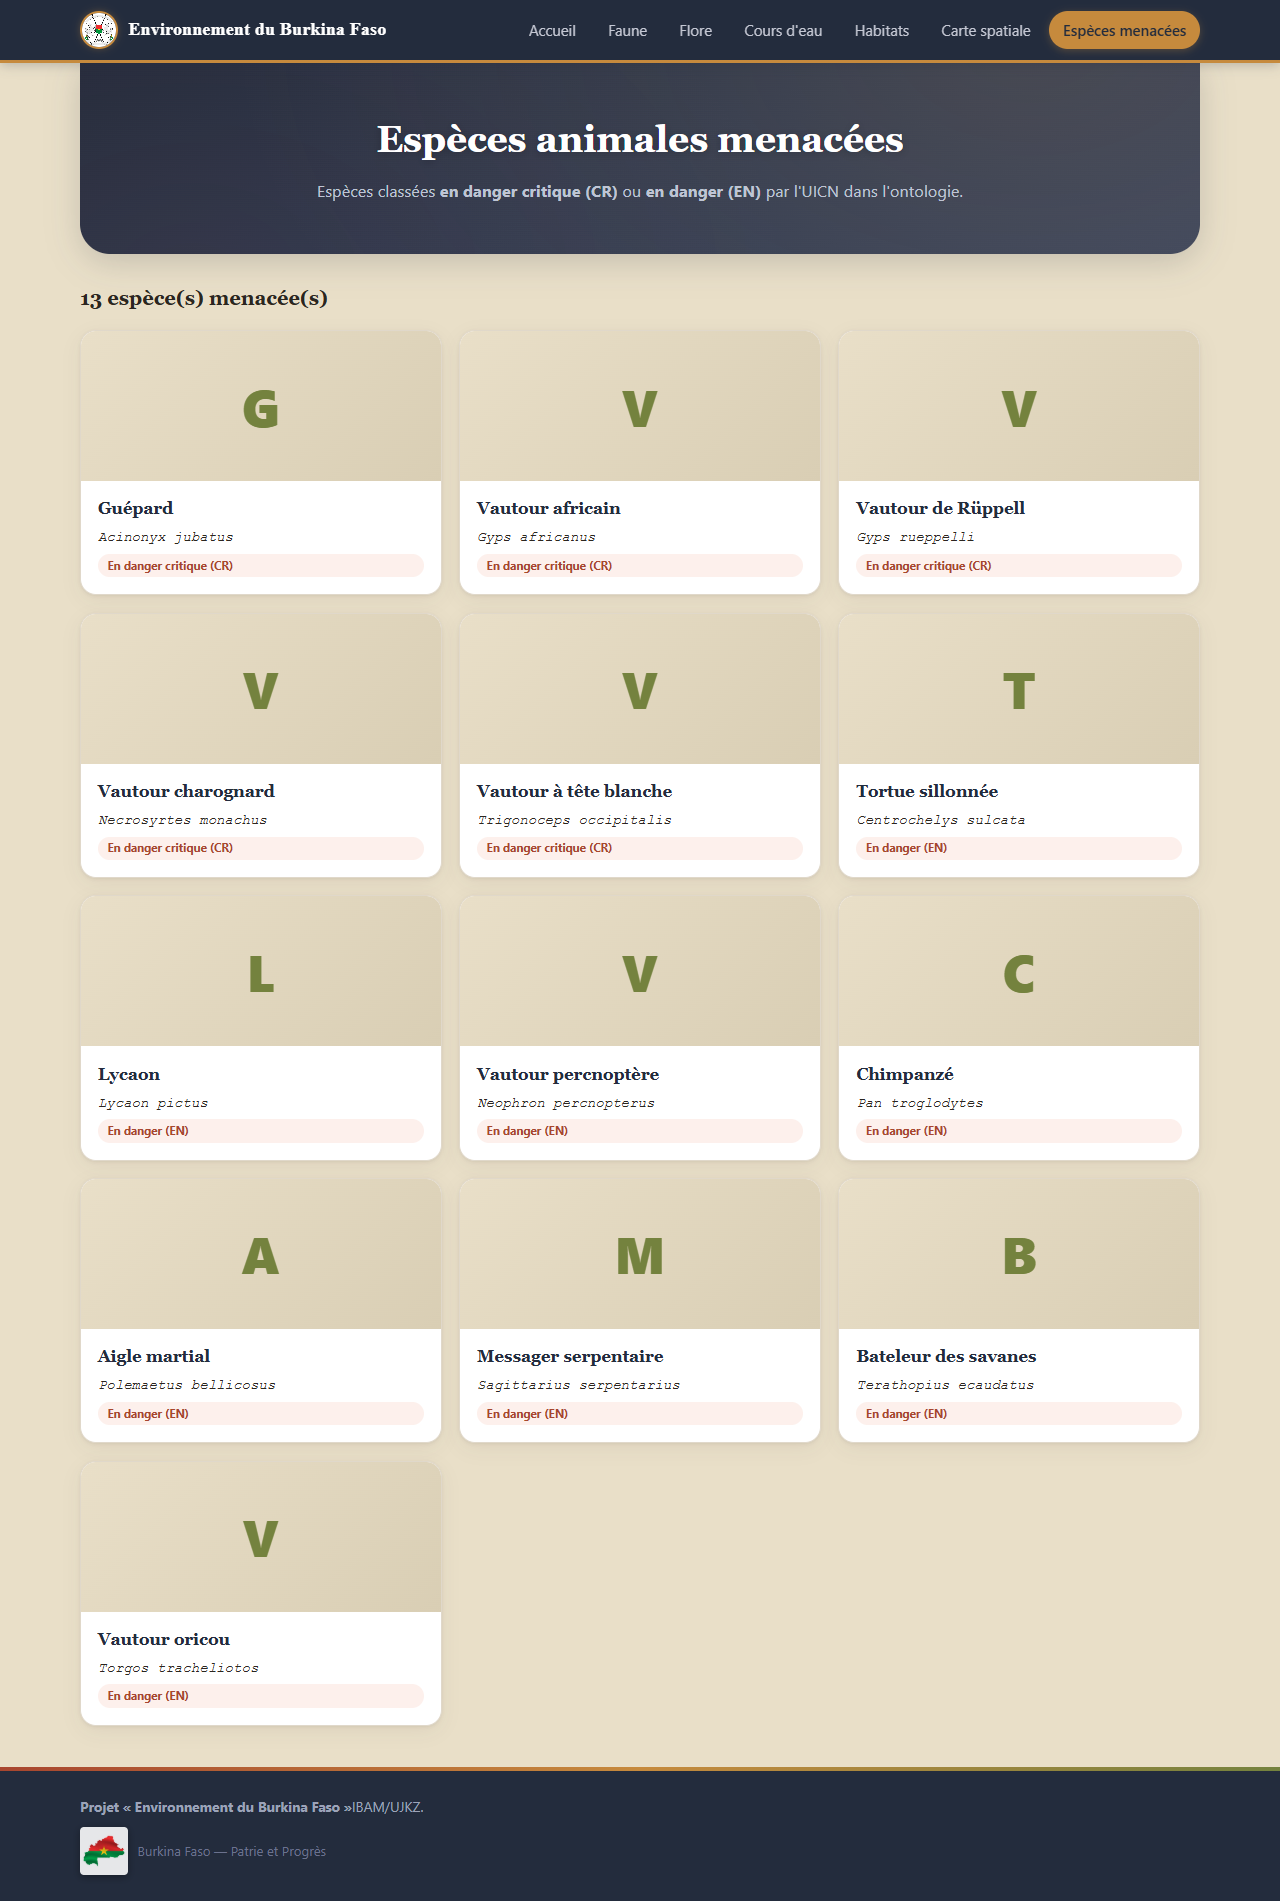
\includegraphics[width=\textwidth]{12_menacees.png}
\caption[Page « Espèces menacées » (statuts CR/EN)]{Page « Espèces menacées » : les 13 espèces animales classées en danger critique (CR) ou en
danger (EN) par l'UICN, avec le statut affiché en badge coloré.}
\end{figure}

% ======================= CHAPITRE 6 =======================
\chapter{Résolution des problèmes}

\begin{table}[H]
\centering
\caption{Problèmes fréquents et solutions}
\begin{tabular}{@{}p{4.0cm}p{5.6cm}p{5.0cm}@{}}
\hline
\tete{Symptôme} & \tete{Cause probable} & \tete{Solution} \\
\hline
\rowcolor{grisfond} \texttt{python} n'est pas reconnu & Python absent ou hors du PATH & Réinstaller Python en cochant \textbf{Add Python to PATH} ; ou utiliser \texttt{py} sous Windows \\
\rowcolor{grisfond} Listes vides ou erreur 500 & Fuseki n'est pas démarré & Lancer \texttt{fuseki-server}, vérifier \url{http://localhost:3030} \\
\rowcolor{grisfond} API en erreur 404 & Le jeu de données ne s'appelle pas \texttt{environnement} & Renommer le dataset dans Fuseki \\
\rowcolor{grisfond} « Port 5000 déjà utilisé » & Une autre instance de l'application tourne & Fermer l'ancien terminal, ou changer le port dans \texttt{app.py} \\
\rowcolor{grisfond} Carte sans tuiles & Connexion Internet absente & Ouvrir une connexion Internet, actualiser la page \\
\rowcolor{grisfond} Ontologie introuvable au lancement & Le fichier \texttt{.owx} n'a pas été chargé & Recharger l'ontologie dans le dataset \texttt{environnement} (chapitre~3) \\
\rowcolor{grisfond} macOS refuse de lancer Fuseki & Sécurité Gatekeeper & Clic droit sur \texttt{fuseki-server} puis « Ouvrir » \\
\rowcolor{grisfond} Recherche sans résultat & Moins de 2 caractères saisis & Saisir au moins deux caractères (insensibles aux accents) \\
\hline
\end{tabular}
\end{table}

\section{Accès en ligne}

L'application est également déployée sur le cloud, permettant d'y accéder directement depuis un
navigateur sans aucune installation locale. Deux plateformes d'hébergement ont été retenues :

\begin{itemize}
\item \textbf{Fly.io} (recommandé) --- hébergement stable, sans mise en veille, HTTPS automatique.
      L'application est accessible à l'adresse suivante :

      \url{https://burkina-environnement.fly.dev}

\item \textbf{Render} --- hébergement complémentaire, avec mise en veille au bout d'une
      inactivité. L'application est accessible à l'adresse suivante :

      \url{https://burkina-environnement.onrender.com}
\end{itemize}

\noindent Ces deux instances sont synchronisées avec le dépôt Git du projet : chaque mise à jour
pushée sur la branche \texttt{main} est automatiquement reconstruite et redéployée.

% ======================= CHAPITRE 7 =======================
\chapter{Conclusion}

L'application « Environnement du Burkina Faso » est autonome une fois ses deux composants démarrés :
le triplestore \textbf{Apache Jena Fuseki} (chargé avec l'ontologie \texttt{burkina-environnement}) et
l'application \textbf{Flask} (\texttt{python app.py}). La procédure complète tient en quatre étapes :
installer Java, démarrer Fuseki, créer le jeu de données \texttt{environnement} et charger
l'ontologie, puis installer les dépendances Python et lancer \texttt{app.py}. Toutes les
fonctionnalités (recherches, filtres, fiches, carte GeoSPARQL) reposent sur des requêtes SPARQL
interrogeant l'ontologie en temps réel, garantissant la cohérence entre les données et l'interface.
L'application est également accessible en ligne via les plateformes Fly.io et Render
(voir §~6.2), ce qui permet de la tester sans aucune installation locale.

% ======================= ANNEXES =======================
\appendix
\chapter{Arborescence du projet}

\begin{verbatim}
app_web_semanique/
|-- app.py
|-- requirements.txt
|-- ontologie_environnement.owx
|-- ontologie_environnement.rdf
|-- backend/
|   |-- sparql.py          # client SPARQL (endpoint Fuseki)
|   |-- commun.py          # statistiques, recherche globale, filtre Burkina
|   |-- faune.py
|   |-- flore.py
|   |-- cours_eau.py
|   `-- habitat.py
|-- web/                   # routes Flask (pages + APIs JSON)
|   |-- accueil.py
|   |-- faune.py
|   |-- flore.py
|   |-- hydro.py
|   |-- carte.py
|   `-- habitat.py
|-- templates/             # gabarits HTML (Jinja2)
|-- static/
|   |-- css/style.css
|   `-- js/                # scripts JavaScript des pages
`-- Manuel_Utilisation/    # present manuel (source LaTeX + captures)
\end{verbatim}

\section{Configuration du endpoint SPARQL}

Le fichier \texttt{backend/sparql.py} définit l'adresse du triplestore :

\begin{lstlisting}
ENDPOINT = "http://localhost:3030/environnement/query"
\end{lstlisting}

\noindent Si le jeu de données Fuseki porte un autre nom, adapter uniquement cette ligne.

\section{Requêtes de vérification}

Nombre d'espèces animales :

\begin{lstlisting}
PREFIX en: <http://www.ibam-ujkz.bf/ontologies/burkina-environnement#>
SELECT (COUNT(?s) AS ?n) WHERE { ?s a en:EspeceAnimale }
\end{lstlisting}

Cinq premiers cours d'eau :

\begin{lstlisting}
PREFIX en: <http://www.ibam-ujkz.bf/ontologies/burkina-environnement#>
SELECT ?nom WHERE { ?s a en:CoursDEau ; en:nom ?nom } LIMIT 5
\end{lstlisting}

\section{Récapitulatif des adresses}

\begin{table}[H]
\centering
\caption{Récapitulatif des adresses}
\begin{tabular}{@{}p{5.8cm}p{9.0cm}@{}}
\hline
\tete{Élément} & \tete{Adresse} \\
\hline
\rowcolor{grisfond} Application en ligne (Fly.io) & \url{https://burkina-environnement.fly.dev} \\
\rowcolor{grisfond} Application en ligne (Render) & \url{https://burkina-environnement.onrender.com} \\
\rowcolor{grisfond} Interface de gestion Fuseki & \url{http://localhost:3030} \\
\rowcolor{grisfond} Endpoint SPARQL & \url{http://localhost:3030/environnement/query} \\
\rowcolor{grisfond} Application (accueil) & \url{http://127.0.0.1:5000} \\
\rowcolor{grisfond} Faune & \url{http://127.0.0.1:5000/faune} \\
\rowcolor{grisfond} Flore & \url{http://127.0.0.1:5000/flore} \\
\rowcolor{grisfond} Cours d'eau & \url{http://127.0.0.1:5000/cours-deau} \\
\rowcolor{grisfond} Habitats & \url{http://127.0.0.1:5000/habitats} \\
\rowcolor{grisfond} Carte spatiale & \url{http://127.0.0.1:5000/carte} \\
\rowcolor{grisfond} Espèces menacées & \url{http://127.0.0.1:5000/menacees} \\
\hline
\end{tabular}
\end{table}

\end{document}
